\documentclass[crop, tikz]{standalone}

\usepackage{tikz}
\usepackage{amsmath}
\usepackage{amssymb}
\usepackage[mode=buildnew]{standalone}

\definecolor{mred}{RGB}{214,39,40}

\begin{document}
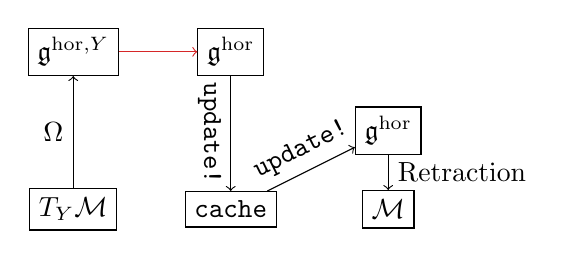
\begin{tikzpicture}
    \node[rectangle, draw] (TYM)   at (0, 0) {$T_Y\mathcal{M}$};
    \node[rectangle, draw] (ghorY) at (0, 2) {$\mathfrak{g}^{\mathrm{hor},Y}$};
    \node[rectangle, draw] (ghor)  at (2, 2) {$\mathfrak{g}^{\mathrm{hor}}$};
    \node[rectangle, draw] (cache) at (2, 0) {$\mathtt{cache}$};
    \node[rectangle, draw] (ghor2) at (4, 1) {$\mathfrak{g}^\mathrm{hor}$};
    \node[rectangle, draw] (M)	   at (4, 0) {$\mathcal{M}$};

    \draw[->] (TYM) -- (ghorY) node[pos=.5, left] {$\Omega$};
    \draw[->, mred] (ghorY) -- (ghor);
    \draw[->] (ghor) -- (cache) node[pos=.5, sloped, below] {\texttt{update!}};
    \draw[->] (cache) -- (ghor2) node[pos=.5, sloped, above] {\texttt{update!}};
    \draw[->] (ghor2) -- (M) node[pos=.5, right] {Retraction};
\end{tikzpicture}
\end{document}